\chapter{Principy kontejnerové virtualizace} \label{chp:kontejner}
První bod této kapitoly se zabývá obecnou historií kontejnerů. K vyjasnění principů pro kontejnerovou virtualizaci je třeba vysvětlit dva základní pojmy, virtualizaci a kontejner.

\section{Historie kontejnerové virtualizace}
První pokusy o kontejnerizaci pocházejí už z roku 1979, kdy bylo možné pro izolaci aplikací a procesů využít chroot. Tento koncept je ovšem velmi jednoduchý a má svá omezení.
V roce 2000 byl chroot zdokonalen v rámci projektu FREEBSD jails\cite{chroot}, taktéž znám pod jménem Chroot on Steriods\cite{chroot}. Toto řešení již bylo pokročilejší, dokázalo plně izolovat proces, byla zde vyřešena podpora pro networking. Vzhledem k malému rozšíření systému FREEBSD se tento projekt dlouhodobě nepoužíval.

Se svým konceptem kontejnerů se představil také Oracle. Projekt se nazýval solaris zones\cite{solaris_zone} (Solaris Containers). Řešení bylo velmi podobné existujícím kontejnerům s lépe vyřešenými požadavky na file systém a podporou ZFS.
V roce 2005 se začala firma Google potýkat s problémy, jak přenášet své webové služby. Google již nějakou  dobu experimentoval s kontejnery pro tuto potřebu, ale zjistil, že se jedná o nevhodné řešení. Hlavní problém byl výkon, který byl příliš slabý a odezva příliš pomalá na to, aby kontejnery dokázaly pracovat s požadovanými webovými službami.

Ve stejném období začali budoucí pracovníci Googlu experimentovat s linuxovým konceptem postaveným na cgroups (control groups), nazývaným jako procesové kontejnery. Za několik měsíců stejná skupina inženýrů pomocí těchto kontejnerů vyřešila problém se škálovatelností jednotlivých data center Googlu. 
V lednu 2008 byly některé cgroup technologie, které používal Google, přidané do Linuxového jádra, čímž daly základ projektu LXC (LinuX Containers).

V roce 2013 společnosti Google a Parallels odsouhlasily spolupráci. Výsledkem bylo vydání Linuxového jádra ve verzi 3.8\cite{gp_38}, které obsahovalo jejich linuxové virtualizační technologie vytvořené těmito společnostmi. Tyto technologie pomohly o několik let později k vzniku technologie Docker.

Docker se poprvé výrazněji prosadil v roce 2013 a ukázal, jakým způsobem může být práce s aplikacemi v kontejnerech na linuxovém jádru výrazně usnadněna. Otcem Dockeru je Solomon Hykes, který položil základ projektu uvnitř firmy dotCloud. Za podpory zaměstnanců dotCloudu se stal nezávislým vývojářem. Docker prakticky změnil celou primární technologii firmy dotCloud a firma se začala specializovat pouze na vývoj tohoto nástroje pro kontejnerizaci.

V roce 2014 firma CoreOS vytvořila zcela nový projekt rkt. Důvodem vzniku projektu bylo dlouhé čekání na schvalování patchů do Dockeru a architektura Dockeru samotná. Rkt je open source a napsán v programovacím jazyce Go.

V roce 2016 představila \cite{windows_container} své kontejnerové řešení i Redmondská firma Microsoft, která má dvě rozdílné technologie kontejnerové virtualizace: Windows Server Containers a Hyper-V Containers. Nutno zmínit, že Microsoft přišel s tímto řešením na trh příliš pozdě, jeho řešení není zatím konkurenceschopné. Velikosti jednotlivých Windows image pro kontejnery jsou obrovské, několik stovek MB, a popírají tak koncept kontejnerů, který si zakládá na tom být co nejmenší.

\section{Kontejner}
Princip kontejneru je už znám desítky let. Kontejnerovou virtualizační technologii lze přirovnat ke klasickým dopravním kontejnerům. Tak jako dopravní kontejnery slouží k přepravě nákladu, tyto kontejnery slouží k doručování aplikací. Koncept kontejnerů je revoluční a nabízí rychlou a dynamickou práci s aplikacemi. Jakmile máme aplikaci v kontejneru, můžeme ji přesouvat a spouštět nezávisle na prostředích, napříč širokým spektrem platforem. Na kontejnery je potřeba nahlížet jinak než na klasickou virtualizaci, kontejnerová virtualizace funguje na rozdílném principu práce se zdroji hosta. Kontejnery dokáží spouštět procesy oddělené od hostitelského stroje pomocí Kernelových cgroups (CPU, GPU, 
disky, síť, atd.), namespaces (systémové zdroje jako: mnt,pid,ipc,users, atd.). 

\section{Virtualizace}
Virtualizaci v nejširším slova smyslu je možné definovat jako emulaci jedné nebo více pracovních stanic nebo serverů bez jediné části hardwaru. To otvírá novou možnost vzít jednomu fyzickému počítači na sebe roli, kterou by za běžných okolností muselo vykonávat více počítačů. V dnešní době už nejde jen o zvyšování a škálování výpočetního výkonu, ale také o sdílení fyzických zdrojů. Tato skutečnost vede také k ekonomickým výhodám, protože už není potřeba tolik hardwaru na infrastrukturu.

Existuje několik různých typů virtualizací, které se používají pro odlišné účely. Lze tvrdit, že v dnešní době počítačů je možno virtualizovat takřka všechno od operačních systémů, přes paměti, disky až po počítačové sítě. Základní stavební jednotkou samotné virtualizace je virtuální stroj(VM), který má obdobné vlastnosti jako skutečný hardwarový počítač. Operační systém tohoto serveru je pak nazýván jako hostitelský. 
 
Virtualizace je v dnešní době základem pro cloudové služby, kde se naplno ukazují její přednosti. Dalším revolučním prvkem, který se s virtualizací potkává a prolíná, je open source kultura. Většina z virtualizačních nástrojů, ať se jedná o kontejnery či virtualizační daemony, jsou open source a jsou vyvíjeny komunitou napříč firmami. V informačních technologiích je běžnou praxí rychlý vývoj, proto vzniklo  několik různých druhů virtualizací.

\subsection{Para-virtualizace}
Para-virtualizace je řešení, které používá technologii hypervisoru. Jedná se o  hybridní řešení. Hypervisor se používá pouze pro částečnou virtualizaci některých hardwarových komponent. Operační systém přistupuje k některým fyzickým hardwarovým komponentům napřímo a zbylé komponenty si přebírá od hypervisoru. Nevýhodou tohoto řešení je skutečnost, že operační systém, který je při této virtualizaci potřeba, musí být modifikovatelný, viz obrázek \ref{fig:paravirt}, proto není možné použít proprietární operační systémy.

\begin{figure}[H]
\begin{centering}
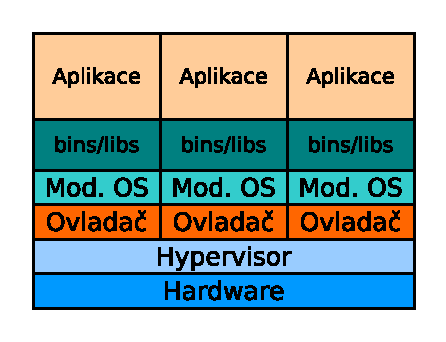
\includegraphics[width=0.8\textwidth]{img/paravirt.pdf}
\par\end{centering}
\caption{Schéma para-virtualizace, zdroj: vlastní tvorba} \label{fig:paravirt}
\end{figure}

\subsection{Plná virtualizace}
Plná virtualizace funguje na principu abstrakce. Všechny fyzické komponenty hostitelského stroje jsou nahrazeny „virtuálním hardwarem“, viz obrázek \ref{fig:fullvirt}. Operační systémy, které fungují na hostitelském počítači nepřistupují přímo na fyzický hardware. Tato skutečnost dává uživateli velké možnosti pro vlastní přizpůsobení virtuálního hardwaru. Vzhledem k této možnosti nejsou aplikace běžící na virtualizovaném systému závislé na fyzicky dostupných komponentech. Další výhodou je fakt, že operační systém, který je použit, nepotřebuje žádné modifikace na rozdíl od para-virtualizace.

\begin{figure}[H]
\begin{centering}
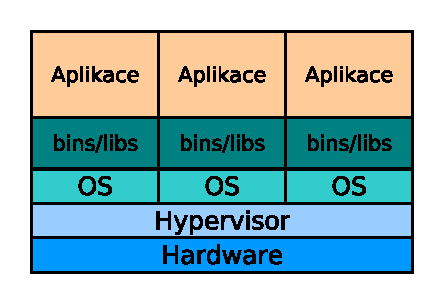
\includegraphics[width=0.8\textwidth]{img/fullvirt.pdf}
\par\end{centering}
\caption{Schéma plné virtualizace, zdroj: vlastní tvorba} \label{fig:fullvirt}
\end{figure}
 
\subsection{Kontejnerová virtualizace}
Kontejnerová virtualizace poskytuje sdílení virtualizačních obrazů operačních systémů skládajících se z root systému, systémových knihoven a spustitelných souborů. Kontejner, poté nahrazuje VM, může být zaveden jako klasický operační systém jenž může být spuštěn, restartován či vypnut. Kontejner může tyto zdroje dynamicky zvýšit či snížit podle potřeby spuštěné aplikace. Aplikace a uživatelé vidí kontejner jako odděleného hosta, znázorněno na obrázku \ref{fig:containervirt}

Kontejnerová virtualizace umožňuje běh jádra s několika odlišnými virtuálními stroji. Na rozdíl od hypervisorové virtualizace nemůže kontejnerový přístup spustit virtuální stroj jako kompletní instanci operačního systému. Kontejnery založené na virtuálních strojích jsou spíše dílčí instance operačních systémů.

Kontejnerová virtualizace nefunguje na celém operačním systému, ale místo toho izoluje systém a nevirtualizuje hardware. Jádro izoluje proces ostatních kontejnerů a řídí jejich zdroje. Všechny kontejnery používají stejné jádro, mají však svůj vlastní file systém, atd.

\begin{figure}[H]
\begin{centering}
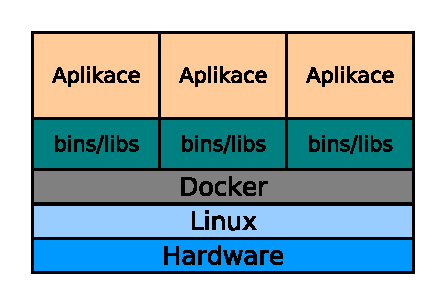
\includegraphics[width=0.8\textwidth]{img/containervirt.pdf}
\par\end{centering}
\caption{Schéma kontejnerové virtualizace, zdroj: vlastní tvorba} \label{fig:containervirt}
\end{figure}

\section{Typy kontejnerové virtualizace}
Kontejnerová virtualizace zažívá obrovský vzestup, spousta firem se snaží kontejnery využít ve svých produkčních prostředích. Rychlý posun kontejnerových technologií v posledních letech lze sledovat převážně díky firmě Docker (původně dotCloud)\cite{dotcloud_docker}. Firma Docker je jedna z firem, která udává směr ve vývoji kontejnerových technologií, a v létě roku 2015 byla oceněna na jednu miliardu amerických dolarů\cite{docker_mil}. 

Kromě technologie od firmy Docker existuje na trhu řada konkurenčních technologií, které z části staví na technologiích Dockeru. Jiné firmy se pokoušejí prosadit se svým vlastním konceptem. S rychlým rozšiřováním kontejnerového trhu přišly obavy o konkurenceschopnost jednotlivých technologií. Technologie Dockeru se objevily na trhu první a mají stále před konkurenčními projekty náskok. Ze strany firem se jedná o technologii, o kterou mají firmy největší zájem, viz obrázek \ref{fig:docker_vs_others}. Podle průzkumu serveru ClusterHQ v roce 2016 jsou kontejnery využívány v produkci v 76 \% dotázaných firem\cite{cluster_vyzkum}.

Díky této skutečnosti vznikla obava, že se z firmy Docker na trhu stane monopol. Z tohoto důvodu byly založeny dvě organizace: OpenContainer Initiative  (OCi) a The Cloud Native Computing Foundation (CNCF). První jmenovaná  je sdružení, které bylo založeno v roce 2015\cite{oci_born} s cílem přinést do kontejnerového světa standardy a dát možnost i jiným firmám podílet se na vývoji kontejnerových technologií, aby všechny kontejnerové projekty měly stejné specifikace pro používané zdroje. CNCF se snaží o větší propagaci kontejnerových technologií a rozšíření se do podvědomí, především v podnikové sféře.

\begin{figure}[H]
\begin{centering}
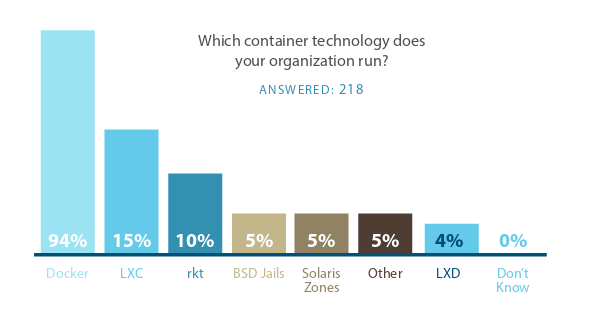
\includegraphics[width=0.8\textwidth]{img/docker_vs_others.png}
\par\end{centering}
\caption{Nejpoužívanější kontejnerové technologie podle serveru ClusterHQ, převzato z \cite{{cluster_vyzkum}}} \label{fig:docker_vs_others}
\end{figure}

V dnešní virtualizaci stále značnou část zastupují VM, avšak mezi technologickými firmami se už VM označují jako legacy technologie. Na rozdíl od klasické virtualizace jsou kontejnery velmi lehkotonážní. Hlavní rozdíl je tak ve smyslu používání. VM můžeme chápat jako celistvý server, na který lze nainstalovat více aplikací a poté obsluhovat více rolí najednou. Ke kontejnerům se musí přistupovat odlišněji. Je potřeba každou službu spustit v odděleném kontejneru a dodržovat tak koncept mikroslužeb. Ve světě kontejnerů je abstrahována celá aplikace. Data produkovaná kontejnerovými aplikacemi nejsou ukládána do kontejnerů ale mimo něj na hostitelský file systém skrze volumy. 


\subsection{Docker}
Docker je platforma zaměřená na kontejnerovou virtualizaci, je publikovaná jako open source, vydaná pod licencí Apache 2.0. Docker není pouze systém, který se zaměřuje na práci s kontejnery. Jedná se o binární balík, který obsahuje i orchestrátory (Compose, Swarm)\cite{docker_1_12}. 

Docker obsahuje nástroje na správu images, pomocí které lze jednotlivé vrstvy image dávat na sebe. Celý koncept images je založen na union mount systému\cite{Docker_OD}. Na obrázku \ref{fig:docker_layers} je znázorněn vrstvící systém, který Docker používá. V tomto vrstvícím systému má pouze vrchní vrstva právo zapisovat, zbytek má pouze právo číst. Tyto images se pak dají šířit pomocí repositáře zvaného Docker Hub, tento repositář funguje na velmi podobném principu jako distribuovaný systém pro správu verzí git. 

Docker je postaven nad ovladačem libcontainer, který ovládá kernel a spravuje systémové zdroje. Libcontainer přišel do Dockeru až s verzí 0.9\cite{docker_lib}, kde nahradil stávající řešení postavené na zdrojích z projektu LXC. Uvnitř Docker kontejneru běží RunC, což je lehkotonážní runtime, který vychází ze standardů OCi. Velkou nevýhodou Dockeru jsou nové verze, které vycházejí nepravidelně každé tři měsíce. Občas se stává, že nová verze není zpětně kompatibilní se starší, tudíž aktualizace je problém zvláště na produkčním prostředí, kde se používají starší a stabilní verze. 

\begin{figure}[H]
\begin{centering}
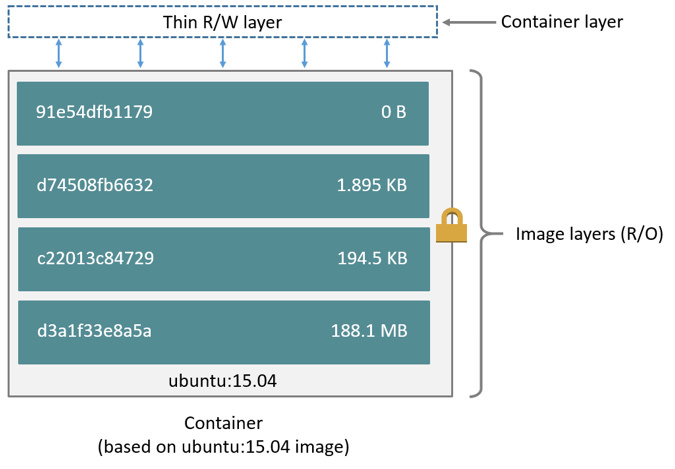
\includegraphics[width=0.7\textwidth]{img/docker_layers}
\par\end{centering}
\caption{Docker vrstvy, převzato z: \cite{Docker_doc_layers} \label{fig:docker_layers}}
\end{figure}

\subsection{Rkt}
Kontejnerová technologie rkt [:rock-it:] je další z řady projektů od firmy CoreOS s otevřeným zdrojovým kódem. Oproti Dockeru rkt není funkční na velkém spektru platforem, nabízí podporu pouze pro Linuxové distribuce. Projekt rkt byl vytvořen a implementuje zmíněné standardy od OCi\cite{coreos_00}. Umožňuje spouštět dva typy images. OCi kompatibilní images vytvořené na základně OCi předpisu a Docker images, které byly vytvořeny konkurenčním řešením. Další odlišnost od konkurenčních řešení je proces model, který dokáže spouštět procesy ve stromové struktuře, je velmi podobný Linuxové struktuře procesů. Rozdíl mezi architekturou Dockeru a rkt je znázorněn na obrázku  \ref{fig:docker_vs_rkt}. 

\begin{figure}[H]
\begin{centering}
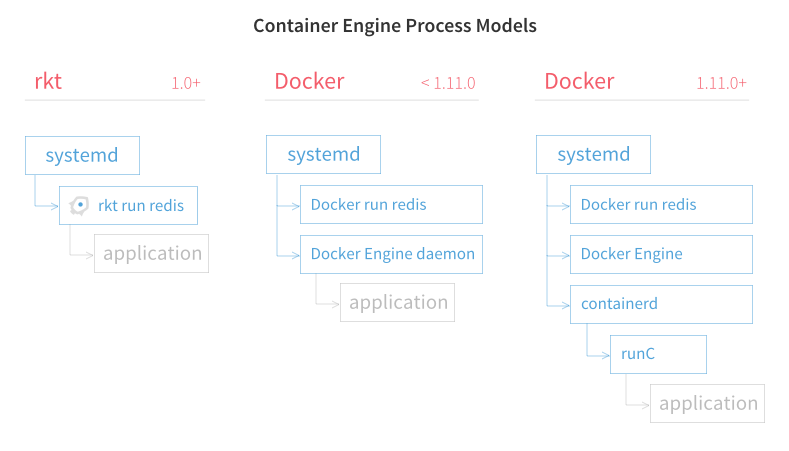
\includegraphics[width=1\textwidth]{img/docker_vs_rkt}
\par\end{centering}
\caption{rkt vs Docker architektura, převzato z: \cite{Docker_vs_rkt} \label{fig:docker_vs_rkt}}
\end{figure}

\subsection{Crio-o}
Cri-o je projekt založený na standardech vytvořených OCi. Zároveň implementuje rozhraní pro kubelet container runtime (CRI). Projekt vzniká pod hlavičkou kubernetes-incubator na serveru github\cite{kube_incubator}. Kubernetes-incubator zastupuje nové projekty, které se týkají Kubernetes a kontejnerů. Projekty nacházející se v incubatoru nejsou na tolik vyspělé, aby mohly být pod oficiální hlavičkou Kubernetes. Projekt Cri-o má stanoven několik hlavních cílů. První z nich je podpora různých typů images založených na standardech OCi. Dalšími jsou managment jednotlivých vrstev těchto images, kontejnerový life-cycle managment a monitorování a správa logů\cite{cri_o_inc}. 

Globální cíl projektu je mít runtime, který umožňuje Kubernetes pomocí CRI implementace spouštět a ovládat kontejnery postavené na standardech od OCi. Cri-o nemá zatím stabilní verzi\cite{cri_o}, takže ho nelze použít v produkčním prostředí.

\section{Výhody kontejnerové virtualizace}
Mezi hlavní výhody patří výkon a škálovatelnost kontejnerů. Hlavní rozdíl mezi kontejnerovou a hypervisorovou virtualizací je, že kontejnery nepoužívají celé VM a mají menší nároky na hardware. Kontejnery běží jako izolované aplikace v rámci operačního systému. Z toho důvodu kontejnerová virtualizace eliminuje potřebu duplikovat určitou funkcionalitu operačního systému, například neduplikuje hardwarová volání a jeden operační systém je zodpovědný za správu všech hardwarových přístupů.
Oproti hypervisorové virtualizaci mají kontejnery limit kolik CPU a paměti bude přiřazeno k operačnímu systému. Kontejnerové řešení by mělo být schopno adresovat všechny volné CPU a RAM paměti pro dané jádro. Vzhledem k tomu, že kontejnery sdílejí operační systém, jsou značně menší než VM. Mohou být tvořeny a spuštěny rychleji než klasická VM. Nabízí tak lepší výkon pro aplikace, které obsahují. Toto řešení je vhodnou volbou, pokud je potřeba nasadit několik desítek až stovek Linuxových hostů.
